\documentclass[10pt,landscape,letter]{article}
\usepackage[landscape,margin=0.5in]{geometry}
\usepackage{multicol}
\usepackage{amsmath,amssymb}
\usepackage{graphicx}
\usepackage{xcolor}
\usepackage{tikz}
\usepackage{booktabs}
\usepackage{enumitem}
\usepackage{fancyhdr}
\usepackage{titlesec}
\usepackage{fancyvrb}

% Compact formatting
\setlength{\parindent}{0pt}
\setlength{\parskip}{2pt}
\setlist[itemize]{leftmargin=*, noitemsep, topsep=0pt}
\setlist[enumerate]{leftmargin=*, noitemsep, topsep=0pt}

% Section formatting
\titleformat{\section}{\normalfont\large\bfseries\color{blue!70!black}}{\thesection}{1em}{}
\titleformat{\subsection}{\normalfont\normalsize\bfseries\color{blue!50!black}}{\thesubsection}{1em}{}
\titlespacing*{\section}{0pt}{6pt}{3pt}
\titlespacing*{\subsection}{0pt}{4pt}{2pt}

% Box for important formulas
\newcommand{\importantbox}[1]{%
  \fcolorbox{blue!50!black}{blue!5}{%
    \parbox{0.90\linewidth}{#1}%
  }%
}

% Red warning box
\newcommand{\warningbox}[1]{%
  \fcolorbox{red!70!black}{red!5}{%
    \parbox{0.90\linewidth}{#1}%
  }%
}

% Green insight box
\newcommand{\insightbox}[1]{%
  \fcolorbox{green!50!black}{green!5}{%
    \parbox{0.90\linewidth}{#1}%
  }%
}

\pagestyle{fancy}
\fancyhf{}
\fancyhead[C]{\raisebox{-8pt}{\textbf{Branched and Cyclic Pathways -- Cheat Sheet V1.0}}}
\fancyfoot[C]{\thepage}
\renewcommand{\headrulewidth}{0.5pt}

\begin{document}

\begin{multicols}{3}

% =============================================================================
\section{Simple Branch Structure}
% =============================================================================

\subsection{Basic Topology}

\begin{center}
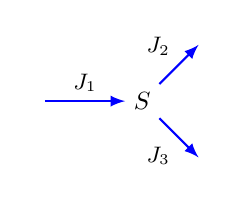
\begin{tikzpicture}[>=latex, scale=0.9, every node/.style={scale=0.9}]
  \node (S0) {};
  \node [right of=S0, node distance=1.5cm] (S1) {$S$};
  \node [above right of=S1, node distance=1.3cm] (S2) {};
  \node [below right of=S1, node distance=1.3cm] (S3) {};

  \draw [->,thick,blue] (S0) -- node[above, black] {\small $J_1$} (S1);
  \draw [->,thick,blue] (S1) -- node[above left, black] {\small $J_2$} (S2);
  \draw [->,thick,blue] (S1) -- node[below left, black] {\small $J_3$} (S3);
\end{tikzpicture}
\end{center}

\subsection{Mass Conservation}

At any branch node with $b$ branches entering and $d$ leaving:
\[
\sum_{i=1}^b v_i - \sum_{j=1}^d v_j = \frac{dS}{dt}
\]

\importantbox{
\textbf{Steady-state constraint:}
\[ J_1 = J_2 + J_3 \]
}

\subsection{Flux Fraction}

Define the flux split:
\begin{align*}
\alpha &= \frac{J_2}{J_1} \quad \text{(fraction through } J_2\text{)} \\[4pt]
1-\alpha &= \frac{J_3}{J_1} \quad \text{(fraction through } J_3\text{)}
\end{align*}

% =============================================================================
\section{Control Coefficients}
% =============================================================================

\subsection{Counting Coefficients}

For a simple branch with 3 enzymes and 1 intermediate:

\begin{center}
\small
\begin{tabular}{@{}ll@{}}
\toprule
\textbf{Type} & \textbf{Count} \\
\midrule
Flux CCs & $3 \times 3 = 9$ \\
Conc CCs & $3 \times 1 = 3$ \\
\textbf{Total} & \textbf{12} \\
\bottomrule
\end{tabular}
\end{center}

\subsection{Control Coefficient Matrix}

\[
\begin{array}{c|ccc}
 & e_1 & e_2 & e_3 \\
\hline
J_1 & C^{J_1}_{e_1} & C^{J_1}_{e_2} & C^{J_1}_{e_3} \\[4pt]
J_2 & C^{J_2}_{e_1} & C^{J_2}_{e_2} & C^{J_2}_{e_3} \\[4pt]
J_3 & C^{J_3}_{e_1} & C^{J_3}_{e_2} & C^{J_3}_{e_3} \\[4pt]
S & C^{S}_{e_1} & C^{S}_{e_2} & C^{S}_{e_3}
\end{array}
\]

% =============================================================================
\section{Summation Theorems}
% =============================================================================

\importantbox{
Each flux has its own summation theorem:
\begin{align*}
C^{J_1}_{e_1} + C^{J_1}_{e_2} + C^{J_1}_{e_3} &= 1 \\
C^{J_2}_{e_1} + C^{J_2}_{e_2} + C^{J_2}_{e_3} &= 1 \\
C^{J_3}_{e_1} + C^{J_3}_{e_2} + C^{J_3}_{e_3} &= 1
\end{align*}
}

And for concentration:
\[ C^{S}_{e_1} + C^{S}_{e_2} + C^{S}_{e_3} = 0 \]

% =============================================================================
\section{Connectivity Theorems}
% =============================================================================

\importantbox{
One connectivity theorem per flux:
\begin{align*}
C^{J_1}_{e_1} \varepsilon^{v_1}_S + C^{J_1}_{e_2} \varepsilon^{v_2}_S + C^{J_1}_{e_3} \varepsilon^{v_3}_S &= 0 \\
C^{J_2}_{e_1} \varepsilon^{v_1}_S + C^{J_2}_{e_2} \varepsilon^{v_2}_S + C^{J_2}_{e_3} \varepsilon^{v_3}_S &= 0 \\
C^{J_3}_{e_1} \varepsilon^{v_1}_S + C^{J_3}_{e_2} \varepsilon^{v_2}_S + C^{J_3}_{e_3} \varepsilon^{v_3}_S &= 0
\end{align*}
}

\vspace{5pt}
\textbf{Problem:} 3 unknowns, only 2 equations (summation + connectivity). Need a third equation!

% =============================================================================
\section{Branch Point Theorems}
% =============================================================================

\subsection{Derivation Strategy}

\textbf{Thought experiment:}
\begin{enumerate}
\item Perturb $e_2$ by $\delta e_2$
\item Compensate with $e_3$ such that $\delta S = 0$
\item Since $\delta S = 0$ and $e_1$ unchanged: $\delta J_1 = 0$
\item Use $\delta v_2 + \delta v_3 = 0$ at branch point
\end{enumerate}

\subsection{Flux Branch Point Theorems}

\importantbox{
\textbf{With respect to $J_1$:}
\[ C^{J_1}_{e_2}(1-\alpha) - C^{J_1}_{e_3}\alpha = 0 \]
}

\textbf{With respect to $J_2$:}
\[ C^{J_2}_{e_1}(1-\alpha) + C^{J_2}_{e_3} = 0 \]

\textbf{With respect to $J_3$:}
\[ C^{J_3}_{e_1}\alpha + C^{J_3}_{e_2} = 0 \]

\subsection{Concentration Branch Point Theorems}

\importantbox{
\[ C^S_{e_2}(1-\alpha) - C^S_{e_3}\alpha = 0 \]
}

Variants:
\begin{align*}
C^S_{e_1}(1-\alpha) + C^S_{e_3} &= 0 \\
C^S_{e_1}\alpha + C^S_{e_2} &= 0
\end{align*}

%\columnbreak

% =============================================================================
\section{Solving for Control Coefficients}
% =============================================================================

\subsection{Matrix Formulation}

Combine summation, connectivity, and branch theorems:
\[
\mathbf{C} \cdot \mathbf{T} = \mathbf{I}
\]

For $J_2$:
\[
\begin{bmatrix}
C^{J_2}_{e_1} & C^{J_2}_{e_2} & C^{J_2}_{e_3}
\end{bmatrix}
\begin{bmatrix}
1 & \varepsilon_1 & 0 \\
1 & \varepsilon_2 & 1-\alpha \\
1 & \varepsilon_3 & 1
\end{bmatrix}
= \begin{bmatrix} 1 & 0 & 0 \end{bmatrix}
\]

\subsection{Explicit Formulas for $J_2$}

Let $D = \varepsilon_2\alpha + \varepsilon_3(1-\alpha) - \varepsilon_1$ (denominator).

\textbf{Note:} $D > 0$ when $\varepsilon_1 < 0$, $\varepsilon_2, \varepsilon_3 > 0$.

\importantbox{
\textbf{Flux control coefficients:}
\begin{align*}
C^{J_2}_{e_1} &= \frac{\varepsilon_2}{D} > 0 \\[6pt]
C^{J_2}_{e_2} &= \frac{\varepsilon_3(1-\alpha) - \varepsilon_1}{D} > 0 \\[6pt]
C^{J_2}_{e_3} &= \frac{-\varepsilon_2(1-\alpha)}{D} < 0
\end{align*}
}

\vspace{10pt}
\importantbox{
\textbf{Concentration control coefficients:}
\begin{align*}
C^{S}_{e_1} &= \frac{1}{D} > 0 \\[6pt]
C^{S}_{e_2} &= \frac{-\alpha}{D} < 0 \\[6pt]
C^{S}_{e_3} &= \frac{-(1-\alpha)}{D} < 0
\end{align*}
}

\vspace{4pt}
\subsection{Sign Patterns}

\begin{center}
\small
\begin{tabular}{@{}lccc@{}}
\toprule
& $e_1$ & $e_2$ & $e_3$ \\
\midrule
$C^{J_2}$ & $+$ & $+$ & $-$ \\
$C^S$ & $+$ & $-$ & $-$ \\
\bottomrule
\end{tabular}
\end{center}

\textbf{Key insight:} $C^{J_2}_{e_3} < 0$ means \textbf{competition} between branches---increasing $e_3$ ``steals'' flux from $J_2$.

% =============================================================================
\section{Branch Point Ultrasensitivity}
% =============================================================================

\subsection{Case 1: Most Flux Through $J_3$}

When $\alpha \to 0$ (small flux through $J_2$):

\begin{center}
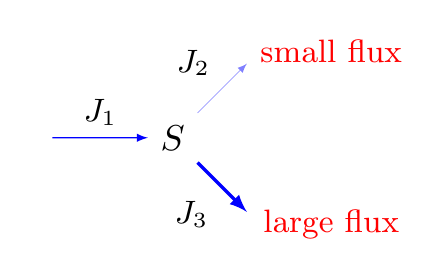
\begin{tikzpicture}[>=latex, scale=1.0, every node/.style={scale=1.3}]
  \node (S0) {};
  \node [right of=S0, node distance=1.3cm] (S1) {$S$};
  \node [above right of=S1, node distance=1.2cm] (S2) {};
  \node [below right of=S1, node distance=1.2cm] (S3) {};

  \draw [->,thin,blue] (S0) -- node[above, black] {\small $J_1$} (S1);
  \draw [->,very thin,blue!50] (S1) -- node[above left, black] {\small $J_2$} (S2);
  \draw [->,very thick,blue] (S1) -- node[below left, black] {\small $J_3$} (S3);

  \node[red, right of=S2, node distance=0.7cm] {\small small flux};
  \node[red, right of=S3, node distance=0.7cm] {\small large flux};
\end{tikzpicture}
\end{center}

\importantbox{
As $\alpha \to 0$:
\begin{align*}
C^{J_2}_{e_2} &\to 1 \\[4pt]
C^{J_2}_{e_3} &\to \frac{\varepsilon_2}{\varepsilon_1 - \varepsilon_3}
\end{align*}
}

\vspace{10pt}
\warningbox{
\textbf{Ultrasensitivity:} Control coefficients can \textbf{greatly exceed 1}!

Example: $C^{J_2}_{e_1} = 8.34$ means 1\% increase in $e_1$ causes 8\% increase in $J_2$.
}

\vspace{4pt}
\textbf{Analogy:} A small stream off a large river---flooding in the river has huge impact on the stream.

\subsection{Case 2: Most Flux Through $J_2$}

When $\alpha \to 1$ (large flux through $J_2$):

\begin{center}
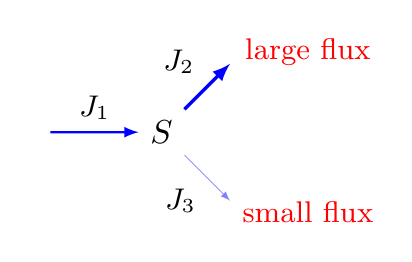
\begin{tikzpicture}[>=latex, scale=1.0, every node/.style={scale=1.2}]
  \node (S0) {};
  \node [right of=S0, node distance=1.3cm] (S1) {$S$};
  \node [above right of=S1, node distance=1.2cm] (S2) {};
  \node [below right of=S1, node distance=1.2cm] (S3) {};

  \draw [->,thick,blue] (S0) -- node[above, black] {\small $J_1$} (S1);
  \draw [->,very thick,blue] (S1) -- node[above left, black] {\small $J_2$} (S2);
  \draw [->,very thin,blue!50] (S1) -- node[below left, black] {\small $J_3$} (S3);

  \node[red, right of=S2, node distance=0.7cm] {\small large flux};
  \node[red, right of=S3, node distance=0.7cm] {\small small flux};
\end{tikzpicture}
\end{center}

As $\alpha \to 1$:
\begin{align*}
C^{J_2}_{e_2} &\to \frac{\varepsilon_1}{\varepsilon_1 - \varepsilon_2} \\[4pt]
C^{J_2}_{e_3} &\to 0
\end{align*}

\insightbox{
Pathway behaves as a \textbf{linear chain} ($J_1 \to J_2$). The minor branch $J_3$ has negligible influence.
}

%\columnbreak

% =============================================================================
\section{Conditions for Ultrasensitivity}
% =============================================================================

\subsection{Requirements}

To maximize sensitivity of $J_2$ at a branch:

\begin{enumerate}
\item \textbf{Asymmetric flux:} Most flux through $J_3$ ($\alpha \ll 1$)

\item \textbf{High $\varepsilon_2$ relative to $\varepsilon_3$:}
\begin{itemize}
\item Positive cooperativity at $E_2$
\item $v_3$ more saturated than $v_2$ ($K_m^{(2)} > K_m^{(3)}$)
\end{itemize}

\item \textbf{Small product inhibition:} $|\varepsilon_1|$ small
\end{enumerate}

\subsection{Extreme Case}

It is possible to arrange kinetics such that:
\begin{itemize}
\item $C^{J_2}_{e_1} = +1$
\item $C^{J_2}_{e_2} = +1$
\item $C^{J_2}_{e_3} = -1$
\end{itemize}

\vspace{5pt}
\insightbox{
\textbf{Every step} is equally ``rate-limiting''! This shows rate limitation is not a simple concept.
}

% =============================================================================
\section{Futile (Substrate) Cycles}
% =============================================================================

\subsection{Structure}

\begin{center}
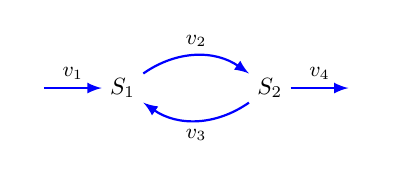
\begin{tikzpicture}[>=latex, scale=0.85, every node/.style={scale=0.85}]
\node (S2) {$S_2$};
\node [left of=S2, node distance=2.2cm] (S1) {$S_1$};

\node [left of=S1, node distance=1.3cm] (Xo) {};
\draw[->,thick,blue] (Xo) -- node[above,black] {\small $v_1$} (S1);

\node [right of=S2, node distance=1.3cm] (X1) {};
\draw[->,thick,blue] (S2) -- node[above,black] {\small $v_4$} (X1);

\draw [->,thick,blue] (S2) to [bend left=35] node[below,black] {\small $v_3$} (S1);
\draw [->,thick,blue] (S1) to [bend left=35] node[above,black] {\small $v_2$} (S2);
\end{tikzpicture}
\end{center}

\textbf{Flux constraint:}
\[ v_1 = v_2 - v_3 = v_4 \]

\textbf{Examples:} Glucose $\leftrightarrow$ G6P, F6P $\leftrightarrow$ F1,6BP

\subsection{Amplification Mechanism}

\importantbox{
\textbf{Maximum amplification:}
\[ \frac{\delta v_1/v_1}{\delta v_2/v_2} = \frac{v_2}{v_1} = 1 + \frac{v_3}{v_1} \]
}

\vspace{4pt}
Higher cycling rate ($v_3$) relative to through flux ($v_1$) gives greater amplification.

\subsection{Numerical Example}

\begin{center}
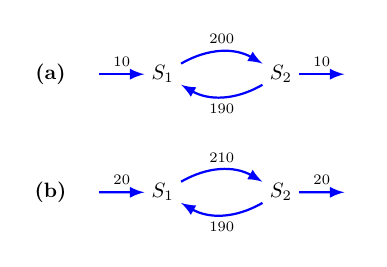
\begin{tikzpicture}[>=latex, scale=0.75, every node/.style={scale=0.75}]
% Reference state
\node at (-3.9,0) {\textbf{(a)}};
\node (S2) {$S_2$};
\node [left of=S2, node distance=2cm] (S1) {$S_1$};
\node [left of=S1, node distance=1.2cm] (Xo) {};
\draw[->,thick,blue] (Xo) -- node[above,black] {\scriptsize $10$} (S1);
\node [right of=S2, node distance=1.2cm] (X1) {};
\draw[->,thick,blue] (S2) -- node[above,black] {\scriptsize $10$} (X1);
\draw [->,thick,blue] (S2) to [bend left=30] node[below,black] {\scriptsize $190$} (S1);
\draw [->,thick,blue] (S1) to [bend left=30] node[above,black] {\scriptsize $200$} (S2);

% Perturbed state
\node at (-3.9,-2) {\textbf{(b)}};
\node[below of=S2, node distance=2cm] (S22) {$S_2$};
\node [left of=S22, node distance=2cm] (S11) {$S_1$};
\node [left of=S11, node distance=1.2cm] (Xoo) {};
\draw[->,thick,blue] (Xoo) -- node[above,black] {\scriptsize $20$} (S11);
\node [right of=S22, node distance=1.2cm] (X11) {};
\draw[->,thick,blue] (S22) -- node[above,black] {\scriptsize $20$} (X11);
\draw [->,thick,blue] (S22) to [bend left=30] node[below,black] {\scriptsize $190$} (S11);
\draw [->,thick,blue] (S11) to [bend left=30] node[above,black] {\scriptsize $210$} (S22);
\end{tikzpicture}
\end{center}

\warningbox{
5\% increase in $v_2$ $\Rightarrow$ \textbf{100\% increase} in $v_1$!

(Assuming $v_3$ unchanged due to saturation)
}

\subsection{MCA Analysis of Cycles}

Flux control coefficient for $J_1$ with respect to $e_2$:
\[
C^{J_1}_{e_2} = \frac{\varepsilon^1_1 \varepsilon^4_2 (1 + v_3/v_1)}{D}
\]

\textbf{Key requirements:}
\begin{enumerate}
\item Product inhibition on $v_1$ ($\varepsilon^1_1 \neq 0$) is \textbf{essential}
\item Small $\varepsilon^3_2$ (weak activation of reverse arm)
\end{enumerate}

\subsection{Condition for High Sensitivity}

When cycling rate $\gg$ through flux:
\[
C^{J_1}_{e_2} \approx \frac{v_2}{v_3 \frac{\varepsilon^3_2}{\varepsilon^4_2} - v_2 \frac{\varepsilon^2_1}{\varepsilon^1_1}}
\]

Maximal when:
\[
\frac{\varepsilon^3_2}{\varepsilon^4_2} + \frac{\varepsilon^2_1}{\varepsilon^1_1} \ll 1
\]

\textbf{Meaning:}
\begin{itemize}
\item $S_2$ activates $v_4$ more than $v_3$
\item $S_1$ inhibits $v_1$ more than it activates $v_2$
\end{itemize}

% =============================================================================
\section{Summary}
% =============================================================================

\begin{center}
\small
\begin{tabular}{@{}p{2.2cm}p{4.5cm}@{}}
\toprule
\textbf{Feature} & \textbf{Key Point} \\
\midrule
Branch theorem & Third equation needed to solve system \\[4pt]
Competition & $C^{J_i}_{e_j} < 0$ for competing branch \\[4pt]
Ultrasensitivity & $|C| \gg 1$ when minor branch observed \\[4pt]
Linear limit & $\alpha \to 1$: pathway becomes chain \\[4pt]
Futile cycles & Amplification $= 1 + v_3/v_1$ \\
\bottomrule
\end{tabular}
\end{center}

\vfill
\hrule
\vspace{3pt}
\footnotesize
\textit{Based on: H.M. Sauro, ``Systems Biology: An Introduction to Metabolic Control Analysis'', \today}

\end{multicols}
\end{document}
